% !TeX root = ../tfg.tex
% !TeX encoding = utf8

\chapter{Conceptos y estado del arte}

\section{Conceptos de aprendizaje automático}


\section{Visión artificial}

Como hemos comentado brevemente en la sección anterior, la \textbf{visión artificial} es la rama de la La visión artificial es una rama de la Inteligencia Artificial cuyo objetivo es comprender el mundo que percibimos a partir de una o más imágenes y reconstruir propiedades suyas como su forma, iluminación o distribución de colores. Su objetivo final es desarrollar sistemas que puedan interpretar y comprender el entorno visual de manera efectiva.

La visión artificial es un campo en constante evolución, que abarca una amplia variedad de problemas y aplicaciones, desde la automatización de procesos industriales hasta la asistencia a personas con discapacidad. Sin embargo, las principales áreas de investigación en este campo son las siguientes:

\begin{itemize} 
	\item \textbf{Clasificación de objetos}: identificar y categorizar objetos en una imagen, lo que es fundamental en aplicaciones como la detección de objetos en imágenes de seguridad o la clasificación de productos en una tienda en línea. 
	\item \textbf{Generación de imágenes}: crear imágenes a partir de modelos o datos, lo que tiene aplicaciones en la creación de gráficos 3D, la síntesis de imágenes para la publicidad o la creación de contenido en redes sociales. 
	\item \textbf{Reconstrucción de entornos 3D}: reconstruir entornos tridimensionales a partir de imágenes 2D, lo que es fundamental en aplicaciones como la creación de modelos 3D de edificios o la planificación de rutas en un entorno desconocido. 
	\item \textbf{Detección de objetos}: detectar la presencia de objetos en una imagen, lo que es fundamental en aplicaciones como la seguridad en espacios públicos o la detección de anomalías en la producción industrial. 
	\item \textbf{Segmentación de imágenes}: dividir una imagen en regiones significativas, lo que es fundamental en aplicaciones como la medicina, la agricultura o la minería. 
\end{itemize}

En este trabajo, nos enfocaremos en el marco de clasificación de imágenes, que es un problema de aprendizaje automático fundamental en la visión artificial. Nuestro objetivo es analizar cómo diferentes modelos de redes neuronales convolucionales se comportan en diferentes conjuntos de datos y condiciones.

\section{Redes neuronales artificiales}

\subsection{Neuronas biológicas}

Las neuronas biológicas son células nerviosas que se encuentran en el cerebro y otros órganos del sistema nervioso. Estas células son capaces de recibir y enviar señales eléctricas, lo que les permite comunicarse entre sí y procesar información.

Las neuronas biológicas están compuestas por tres partes principales: el soma, la dendrita y el axón. El soma es la parte central de la neurona que contiene el núcleo y el citoplasma. La dendrita es la parte que recibe las señales eléctricas de otras neuronas. El axón es la parte que transmite las señales eléctricas a otras neuronas o a los músculos.

Las neuronas biológicas también tienen una función de activación, que es la función que determina cómo se comporta la neurona en respuesta a las señales eléctricas que recibe. La función de activación es una función escalera, que es una función que se activa cuando la suma de las entradas es mayor que un umbral.

Las neuronas biológicas también tienen sinapsis, que son las conexiones entre las neuronas que permiten la comunicación entre ellas. Las sinapsis se pueden dividir en dos tipos: sinapsis excitadoras y sinapsis inhibitorias. Las sinapsis excitadoras aumentan la probabilidad de que la neurona se active, mientras que las sinapsis inhibitorias disminuyen la probabilidad de que la neurona se active.

\subsection{Redes neuronales artificiales}

Las neuronas biológicas han inspirado la creación de las redes neuronales artificiales. Los biólogos y los matemáticos han estudiado las neuronas biológicas y han desarrollado modelos matemáticos para simular su comportamiento. Estos modelos han sido utilizados para crear redes neuronales artificiales que pueden aprender y adaptarse a nuevos datos.

Las redes neuronales artificiales se basan en la idea de que las neuronas biológicas se comunican entre sí a través de sinapsis. Las redes neuronales artificiales también tienen una función de activación que determina cómo se comporta la neurona en respuesta a las entradas. Sin embargo, las redes neuronales artificiales no tienen sinapsis en el sentido biológico, sino que utilizan matrices de pesos para representar las conexiones entre las neuronas.

Dentro de los distintos modelos de aprendizaje automático, nosotros trabajaremos con redes neuronales artificiales.

\begin{definicion} 
	Sea $w \in \mathbb{R}^d$, $d \in \mathbb{N}$, y $\theta: \mathbb{R} \rightarrow \mathbb{R}$ una función escalar conocida como \textbf{función de activación}. Entonces, una \textbf{neurona} se define como una función $f: \mathbb{R}^d \rightarrow \mathbb{R}$ de la siguiente manera 
	\begin{equation} 
		f(x, w) = \theta \left( \sum_{i=1}^{d} w_i x_i \right), \quad \forall x, w \in \mathbb{R}^d. 
	\end{equation} 
\end{definicion}

Una \textit{neurona} es la unidad fundamental de procesamiento, que aplica una función de activación $\theta$ a la suma ponderada de sus entradas, representadas por los pesos $w$. En una arquitectura de red, las neuronas se agrupan en \textbf{capas}. La \textbf{profundidad} de una red se refiere al número de capas ocultas entre la entrada y la salida, y la \textbf{anchura} se refiere al número de neuronas en una capa individual. Cada capa transfiere su salida, transformada por la función de activación, a la siguiente capa. Las \textbf{conexiones} entre capas están definidas por matrices de peso $W_t$, y el término \textbf{bias}, que suele representarse añadiendo un uno al vector de entrada de cada capa, permite ajustar la salida de la función de activación.

\begin{definicion}
	Sea $T \in \mathbb{N}$ y $d = \{d_0,d_1,\ldots,d_T\} \in \mathbb{N}^{T+1}$. Sea $w = \{W_1,\ldots,W_T\}$ con $W_t \in \mathbb{R}^{(d_{t-1}+1) \times d_t}$ una matriz de pesos y $\theta = \{\theta_t: \mathbb{R} \rightarrow \mathbb{R} \}_{t=1,\ldots,T}$ una colección de funciones escalares. Dado un vector de características de entrada $x \in \mathbb{R}^{d_0}$, consideremos la siguiente secuencia:
	\begin{equation}
		x_0 = \begin{bmatrix}
			1 \\
			x 
		\end{bmatrix},
		\quad x_t = \begin{bmatrix}
			1 \\
			\theta_t(W_t^{\top}x_{t-1})
		\end{bmatrix}, \quad t = 1,\ldots,T-1,
		\quad x_T = \theta_T(W_T^{\top}x_{T-1}).
	\end{equation}
	
	Entonces, una red neuronal hacia adelante se determina por $(T,d,\theta,w)$ e implementa la función $h_{T,d,\theta}(x, w) : \mathbb{R}^{d_0} \rightarrow \mathbb{R}^{d_T}$, donde $h_{T,d,\theta}(x, w) = x_T$.
\end{definicion}

\begin{center}
\def\layersep{2.5cm}
\begin{tikzpicture}[shorten >=1pt,->,draw=black!50, node distance=\layersep]
	\tikzstyle{every pin edge}=[<-,shorten <=1pt]
	\tikzstyle{neuron}=[circle,fill=black!25,minimum size=17pt,inner sep=0pt]
	\tikzstyle{input neuron}=[neuron, fill=green!50];
	\tikzstyle{output neuron}=[neuron, fill=red!50];
	\tikzstyle{hidden neuron}=[neuron, fill=blue!50];
	\tikzstyle{annot} = [text width=4em, text centered]
	
	% Draw the input layer nodes
	\foreach \name / \y in {1,...,4}
	% This is the same as writing \foreach \name / \y in {1/1,2/2,3/3,4/4}
	\node[input neuron, pin=left:Input \#\y] (I-\name) at (0,-\y) {};
	
	% Draw the hidden layer nodes
	\foreach \name / \y in {1,...,5}
	\path[yshift=0.5cm]
	node[hidden neuron] (H-\name) at (\layersep,-\y cm) {};
	
	% Draw the output layer node
	\node[output neuron,pin={[pin edge={->}]right:Output}, right of=H-3] (O) {};
	
	% Connect every node in the input layer with every node in the
	% hidden layer.
	\foreach \source in {1,...,4}
	\foreach \dest in {1,...,5}
	\path (I-\source) edge (H-\dest);
	
	% Connect every node in the hidden layer with the output layer
	\foreach \source in {1,...,5}
	\path (H-\source) edge (O);
	
	% Annotate the layers
	\node[annot,above of=H-1, node distance=1cm] (hl) {Hidden layer};
	\node[annot,left of=hl] {Input layer};
	\node[annot,right of=hl] {Output layer};
\end{tikzpicture}
\end{center}

\subsection{Optimización de redes neuronales}

La optimización en redes neuronales es un componente crítico en el entrenamiento de estos modelos, centrado en la minimización de una función de coste o pérdida, $J(w)$. La función de pérdida evalúa la discrepancia entre las salidas predichas por la red y los valores reales o esperados. Mediante algoritmos de optimización, buscamos encontrar el conjunto de pesos $w$ que minimice esta función de pérdida. Los métodos de optimización basados en el gradiente utilizan la retropropagación para calcular los gradientes de la función de pérdida respecto a los pesos, y así realizar la actualización de los mismos.

El algoritmo de \textbf{descenso del gradiente} es el enfoque más básico de optimización, donde los pesos se actualizan en la dirección opuesta al gradiente de la función de coste:
\begin{equation}
	w_{nuevo} = w_{viejo} - \alpha \nabla J(w_{viejo}),
\end{equation}
con $\alpha$ representando la tasa de aprendizaje. \textbf{Adagrad} es una evolución de este método que adapta la tasa de aprendizaje de cada parámetro, permitiendo actualizaciones más grandes para parámetros infrecuentes y más pequeñas para los frecuentes. Adagrad se define como:
\begin{equation}
	w_{nuevo} = w_{viejo} - \frac{\alpha}{\sqrt{G_{t} + \epsilon}} \odot \nabla J(w_{viejo}),
\end{equation}
donde $G_{t}$ es una matriz diagonal donde cada elemento de la diagonal es la suma de los cuadrados de los gradientes para cada parámetro hasta el paso $t$, y $\epsilon$ es un término de suavizado para evitar la división por cero.

\textbf{RMSprop} modifica Adagrad para mejorar su rendimiento manteniendo un promedio móvil del cuadrado de los gradientes. Esto ajusta la tasa de aprendizaje de manera más adecuada para problemas a largo plazo:
\begin{equation}
	v_{t} = \beta v_{t-1} + (1 - \beta)\nabla J(w_{viejo})^2,
\end{equation}
\begin{equation}
	w_{nuevo} = w_{viejo} - \frac{\alpha}{\sqrt{v_{t} + \epsilon}} \odot \nabla J(w_{viejo}),
\end{equation}
donde $v_{t}$ es el promedio móvil de los gradientes cuadrados y $\beta$ es un factor de descuento que determina la ponderación de la media móvil.

\textbf{Adam} (\textit{Adaptive Moment Estimation}) combina las ideas detrás de momentum y RMSprop. Mantiene estimaciones de los primeros y segundos momentos de los gradientes para ajustar la tasa de aprendizaje de cada parámetro de manera individual:
\begin{equation}
	m_{t} = \beta_1 m_{t-1} + (1 - \beta_1)\nabla J(w_{viejo}),
\end{equation}
\begin{equation}
	v_{t} = \beta_2 v_{t-1} + (1 - \beta_2)(\nabla J(w_{viejo})^2),
\end{equation}
\begin{equation}
	\hat{m}_{t} = \frac{m_{t}}{1 - \beta_1^t},
\end{equation}
\begin{equation}
	\hat{v}_{t} = \frac{v_{t}}{1 - \beta_2^t},
\end{equation}
\begin{equation}
	w_{nuevo} = w_{viejo} - \frac{\alpha}{\sqrt{\hat{v}_{t} + \epsilon}} \odot \hat{m}_{t},
\end{equation}
donde $m_{t}$ y $v_{t}$ son estimaciones del primer y segundo momento respectivamente, $\hat{m}_{t}$ y $\hat{v}_{t}$ son sus correcciones sesgadas, y $\beta_1$, $\beta_2$ son tasas de decaimiento exponencial para los momentos estimados.

La selección del algoritmo de optimización es una decisión clave que puede variar dependiendo de la naturaleza del problema y el tipo de red neuronal que se está entrenando. Adam es especialmente popular en la comunidad de aprendizaje profundo debido a su robustez y buen desempeño en una amplia variedad de problemas.

\subsection{Funciones de activación}

Las funciones de activación $\theta$ son un componente esencial en el diseño de redes neuronales artificiales, ya que introducen no linealidades en el modelo, lo que permite a la red aprender y modelar relaciones complejas en los datos. Sin estas funciones, la red no sería capaz de resolver tareas que van más allá de la mera regresión lineal. En términos matemáticos, una función de activación toma una entrada $z$, que es el resultado de la suma ponderada de las entradas de la neurona, y produce una salida $\theta(z)$ que se transmite a la siguiente capa o como parte de la salida final de la red.

La función de activación \textbf{sigmoide} es una de las primeras en ser utilizadas y se define como:
\begin{equation}
	\theta(z) = \frac{1}{1 + e^{-z}}.
\end{equation}
Esta función tiene una curva en forma de 'S' y transforma los valores de entrada a un rango entre 0 y 1, lo que la hace especialmente útil para problemas de clasificación binaria.

En las aplicaciones modernas, la función de activación \textbf{\textit{Rectified Linear Unit}} (ReLU) se ha convertido en una opción popular debido a su simplicidad y eficiencia en la convergencia durante el entrenamiento. La ReLU se define como:
\begin{equation}
	\theta(z) = \max(0, z).
\end{equation}
La ReLU mantiene los valores positivos intactos mientras que anula los valores negativos, lo que acelera la convergencia y reduce el riesgo de desaparición del gradiente.

Otra función comúnmente utilizada es la \textbf{tangente hiperbólica}, o $\tanh$, que escala la salida a un rango entre -1 y 1. Su expresión matemática es:
\begin{equation}
	\theta(z) = \tanh(z) = \frac{2}{1 + e^{-2z}} - 1.
\end{equation}
La naturaleza centrada en cero de la función tanh facilita la modelización en ciertos tipos de problemas en los que se espera que las salidas estén normalizadas.

Finalmente, la función Softmax es esencial en redes neuronales que realizan clasificación multiclase, ya que convierte un vector de números en una distribución de probabilidad. La función Softmax se define para un vector $z \in \mathbb{R}^K$ como:
\begin{equation}
	\theta(z)_i = \frac{e^{z_i}}{\sum_{k=1}^K e^{z_k}} \quad \text{para } i = 1, \ldots, K.
\end{equation}
Cada componente de la salida representa la probabilidad de que la entrada pertenezca a una de las $K$ clases distintas.

Cada una de estas funciones de activación juega un papel crucial en la arquitectura de una red neuronal, y la elección de una sobre otra puede depender del problema específico que se esté abordando, del comportamiento de la red durante el entrenamiento, y de la naturaleza de los datos. La investigación en este campo continúa proponiendo nuevas funciones de activación para mejorar la eficiencia y capacidad de generalización de las redes neuronales.

\begin{figure}
	\centering
	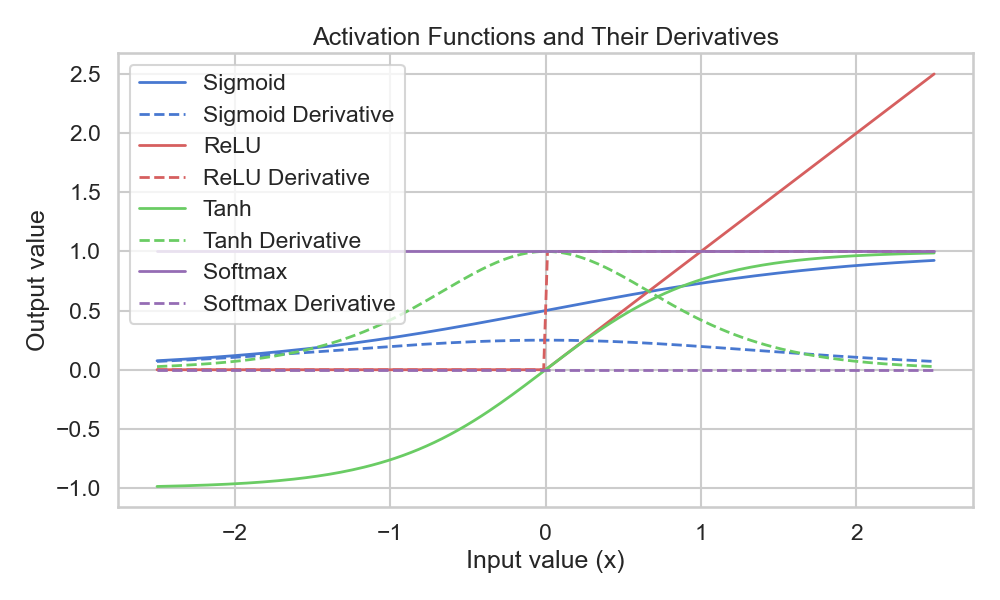
\includegraphics[width=12cm]{img/activation_functions_figure.png}
	\caption{Figura}
\end{figure}

\subsection{Regularización de redes neuronales}

Las técnicas de regularización son cruciales para mejorar la capacidad de generalización de las redes neuronales y prevenir el sobreajuste, que ocurre cuando una red aprende patrones del ruido específico del conjunto de entrenamiento en lugar de las verdaderas relaciones subyacentes. El sobreajuste a menudo resulta en un rendimiento deficiente en datos no vistos. Presentamos aquí algunas de las técnicas de regularización más comunes en el aprendizaje profundo.

La regularización $L1$ y $L2$, a menudo llamadas \textit{Lasso} y \textit{Ridge} respectivamente, son técnicas que modifican la función de coste para penalizar los pesos grandes:
\begin{itemize}
	\item La regularización $L1$ añade un término proporcional a la suma de los valores absolutos de los pesos:
	\begin{equation}
		J_{L1}(w) = J(w) + \lambda \sum_{i} |w_i|,
	\end{equation}
	donde $\lambda$ es el parámetro de regularización.
	
	\item La regularización $L2$ añade un término proporcional a la suma de los cuadrados de los pesos:
	\begin{equation}
		J_{L2}(w) = J(w) + \lambda \sum_{i} w_i^2.
	\end{equation}
\end{itemize}
Estos términos de penalización desincentivan los pesos grandes, llevando a una solución más suave y generalizable.

\textit{Dropout} es una técnica poderosa y ampliamente utilizada que implica desactivar aleatoriamente una proporción de neuronas durante cada iteración del entrenamiento. Este enfoque reduce el sobreajuste al forzar a la red a aprender representaciones redundantes:
\begin{equation}
	h' = h \odot \mathcal{B}(p),
\end{equation}
donde $h$ es la activación de una capa, $\mathcal{B}(p)$ es un vector binario aleatorio donde cada elemento tiene una probabilidad $p$ de ser cero, y $\odot$ denota el producto de Hadamard (elemento a elemento).

El \textit{early stopping} es una forma de regularización basada en la detención del entrenamiento antes de que comience el sobreajuste. Se realiza un seguimiento del error en un conjunto de validación separado y el entrenamiento se detiene cuando el error en este conjunto comienza a aumentar, indicando que la red ha comenzado a aprender el ruido del conjunto de entrenamiento.

Estas técnicas, ya sea de forma independiente o combinada, ayudan a asegurar que las redes neuronales no solo minimicen el error en el conjunto de entrenamiento, sino que también mantengan una buena capacidad de generalización a nuevos datos.


\section{Redes neuronales convolucionales}

Las redes neuronales convolucionales (CNNs) son un tipo de modelo de aprendizaje automático que se han vuelto fundamentales en la visión artificial y el procesamiento de imágenes. Fue introducido por Yann LeCun y sus colaboradores en 1998 y desde entonces ha sido ampliamente utilizado en una variedad de aplicaciones, desde la detección de objetos hasta la segmentación de imágenes.

\subsection{Arquitectura de una CNN}

Una CNN está compuesta por varias capas, cada una de las cuales se encarga de una tarea específica. La primera capa es la capa de convolución, que aplica una función de activación a las entradas y luego se combina con otras capas para formar una representación más compleja. La segunda capa es la capa de pooling, que reduce la dimensionalidad de la entrada y ayuda a reducir la cantidad de parámetros que se necesitan para entrenar la red. La tercera capa es la capa de fully connected, que se encarga de clasificar las entradas.

\subsection{Capas de una CNN}

\subsection{Modelos de CNNs}

\subsection{Ventajas de las CNNs}

Las CNNs tienen varias ventajas que las hacen ideales para la visión artificial. En primer lugar, pueden aprender a detectar patrones complejos en las imágenes, como formas y texturas, lo que las hace ideales para la detección de objetos y la segmentación de imágenes. En segundo lugar, pueden aprender a detectar patrones en diferentes escalas, lo que las hace ideales para la detección de objetos en diferentes tamaños y distancias. Finalmente, las CNNs pueden aprender a detectar patrones en diferentes orientaciones y escenas, lo que las hace ideales para la detección de objetos en diferentes contextos.


\section{Análisis de datos topológico}

\endinput
%--------------------------------------------------------------------
% FIN DEL CAPÍTULO. 
%--------------------------------------------------------------------
